\documentclass[a4paper, oneside]{discothesis}



%%%%%%%%%%%%%%%%%%%%%%%%%%%%%%%%%%%%%%%%%%%%%%%%%%%%%%%%%%%%%%%%%%%%%%%%%%%%%%%%%%%%%%%%%%%%%%%%%
% DOCUMENT METADATA

\thesistype{Semester Thesis} % Master's Thesis, Bachelor's Thesis, Semester Thesis, Group Project
\title{Development and optimization of stretchable conductive fibers for fiber electronics}

\author{Ammar Bin Shaqeel Ahmed}
\email{sammar@student.ethz.ch}

\institute{Laboratory of Biosensors and Bioelectronics \\[2pt]
ETH Zürich}

% Optionally, you can put in your own logo here
%logo{\includegraphics[width=0.2\columnwidth]{figures/disco_logo_faded}}

\supervisors{Dr Jaehong Lee\\[2pt] Prof.\ Dr.\ Janos Vörös }

% Optionally, keywords and categories of the work can be shown (on the Abstract page)
%\keywords{Keywords go here.}
%\categories{ACM categories go here.}

\date{July, 2019}

%%%%%%%%%%%%%%%%%%%%%%%%%%%%%%%%%%%%%%%%%%%%%%%%%%%%%%%%%%%%%%%%%%%%%%%%%%%%%%%%%%%%%%%%%%%%%%%%%

\begin{document}

\frontmatter % do not remove this line
\maketitle

\cleardoublepage


\begin{abstract}
    Stretchable fibers are an important component of stretchable electronics, and especially fiber-based stretchable electronics. Previously the fabrication of highly stretchable conductive fibers through the reduction of silver trifluoroacetate \\(\ch{AgCF3COO}) onto spandex fibers has been  demonstrated with hydrazine hydrate (\ch{N2H4 * 4 H2O)} as a reducing agent. However hydrazine hydrate is highly toxic.
    Here we investigate fabrication using, non-toxic, ascorbic acid (\ch{C6H8O6}) as a reducing agent instead of hydrazine hydrate. 
    We found that the most consistent method for producing conductive fibers was 4 cycles of immersion and reduction, with 30 minute immersion and reduction times. The fabricated fibers displayed a resistance to the order of $10^0~\Omega cm^{-1}$ with the fibers conducting until a strain of $\sim66\%$. This is inferior to the fibers produced by the original process, where the resistance was to the order of $10^{-3}~\Omega cm^{-1}$ with the fibers conducting until a strain of $\sim320\%$. However we are optimistic that fibers can be improved as there were important factors (\textit{PH, Temperature, Catalysts}) that were not explored.
    
    
\end{abstract}

\tableofcontents

\mainmatter % do not remove this line

% Start writing here
\chapter{Introduction}
With improvements in technology, stretchable electronics have found many applications, ranging from supercapacitors~\cite{supercap1,supercap2} and artificial skins~\cite{artifical_skin} to wearable electronics~\cite{jae2015}.

One category of stretchable electronics are planar (2D) devices, but these devices have limited applicability as they cannot easily be woven into textiles or used in non-planar substrates~\cite{planar_electronics,jae2018}.
Hence fiber based stretchable electronics are being studied as an alternative~\cite{jae2015}, which has created a need for conductive fibers that are able to maintain electrical properties under strain. 

There are many different approaches to developing stretchable electronics~\cite{review_stretch}. One approach involves embedding a conductive material (e.g. \ch{Ag} nanoparticles) into non-conducting elastomers thus turning converting them into conducting materials .

In a recent paper, Lee et al~\cite{jae2018}, describe a process for manufacturing stretchable, fiber strain sensors using this approach.
Spandex filaments were first soaked in a Ag precursor, saturating the fiber with \ch{Ag+} ions. The ions were then reduced by hydrazine hydrate (\ch{N2H4 * 4 H2O)} leaving the fiber saturated with conductive Ag nanoparticles.

However hydrazine is carcinogenic and highly toxic~\cite{hydrazine_toxic}. Here we modify the process described above by using ascorbic acid (\ch{C6H8O6}) as a reducing agent instead of the highly toxic hydrazine hydrate (\ch{N2H4 * 4 H2O)}.

\chapter{Fabrication}
\section{Method}
The fibers were manufactured through a two part process:
First, polyurethane fibers were immersed in a precursor solution of 35\% wt \ch{AgCF3COO} dissolved in ethanol for 30 minutes. The fibers quickly become saturated with \ch{Ag+} ions. Then the fibers are removed from the solution and left to dry, allowing the ethanol to evaporate from the fiber, leaving the \ch{Ag+} ions behind.

Second, the fibers are immersed in ascorbic acid (\ch{C6H8O6}) which reduces: \begin{equation}
\ch{2 Ag+ + C6H8O6 <=> 2 Ag + C6H6O6 + 2 H+}
\label{reduction_equation}
\end{equation}

Hence, the fiber becomes saturated with conducting \ch{Ag} nanoparticles. The conductivity of the fiber depends on the density of the \ch{Ag} nanoparticles inside the fiber~\cite{jae2018}. The full protocol is listed in Section \ref{fab_protocol}.

\begin{figure}[ht]
    \centering
    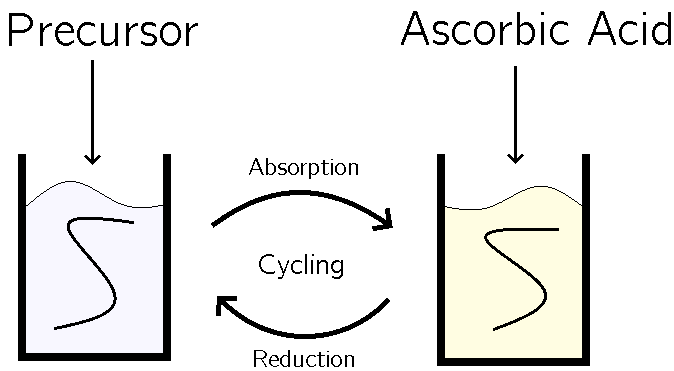
\includegraphics[width=.6\textwidth, keepaspectratio]{figures/cycle.png}
    \caption{Absorption and Reduction Cycle}
\end{figure}

 The resistance/strain relationship of the fiber is then characterised using the protocol described in Section \ref{resistance_protocol}.

\pagebreak

\section{Fabrication Protocol}
\label{fab_protocol}
\begin{enumerate}
    \item Immerse fibers in precursor solution for \textit{Precursor Immersion Time}.
        \begin{itemize}
                \item Narrow vessels are preferred as ethanol evaporates  easily.
            \end{itemize}
    \item Remove and allow to dry. 5 minutes is sufficient.
        \begin{itemize}
            \item It is preferred to dry on tissue paper as the fiber has a tendency to stick to plastic/glass.
        \end{itemize}
    \item Immerse in Ascorbic acid for \textit{Ascorbic Acid Immersion Time}.
        \begin{itemize}
            \item The optimal method is to fill a petri dish with the reducing agent and then place the fiber inside the dish.
            \item It is important that the fiber be \underline{fully immersed} in the reducing agent.
        \end{itemize}
    \item Remove and allow to dry. Here it is important to allow the reducing agent to dry completely before re-immersion, so as not to reduce the precursor solution.
    \item Repeat for \textit{Number of Cycles}.
    \item Measure resistance.
\end{enumerate}

\section{Resistance Measurement Protocol}
\label{resistance_protocol}
\begin{enumerate}
    \item Solder gold foil/wires onto the ends of the sample.
    \item Decide on stretching parameters \textit{Stretching Speed}, \textit{Strain Step} and \textit{Total Strain}.
    \item Measure \textit{Sample Length}.
    \item Place in Zwick stretching machine and clamp, making sure that the wire is vertical.
    \item Attach LCR meter to wires and set machine to continuously record data to excel.
    \item Begin stretching with stretching machine, for \textit{Strain Step} using \textit{Stretching Speed}.
    \item Continue to increment the stretching until the desired \textit{Total Strain}
    is reached, 
    or until the fiber breaks/loses conductivity.
        \begin{itemize}
            \item Note the time at which each stretching step begins.
        \end{itemize}
    \item Process the data to find the strain/resistance relationship.
    
\end{enumerate}

\pagebreak
\section{Parameters}
There are multiple factors that we can optimise for, namely:
\begin{multicols}{2}
\begin{itemize}
    \item \textit{Precursor Concentration}
    \item \textit{Precursor Immersion Time}
    \item \textit{Ascorbic Acid Immersion Time}
    \item \textit{Ascorbic Acid Concentration}
    \item \textit{Number of Cycles}
    \item \textit{Temperature}
    \item \textit{PH}
    \item \textit{Presence of Catalysts}
    \item[\vspace{\fill}]
    \item[\vspace{\fill}]
    \end{itemize}
\end{multicols}

We did not investigate optimal precursor conditions and kept them similar to those of the original process---as the absorption of \ch{Ag+} ions by the fibers saturates at 15\% wt for similar fibers~\cite{cond_shell}; hence the \textit{Precursor Concentration} and the \textit{Precursor Immersion Time} were held constant at 35\% wt and a minimum of 30 minutes, respectively.

\textit{Temperature}, \textit{PH}, and the \textit{Presence of Catalysts} were not investigated, although it is noted in Equation \ref{reduction_equation} that \ch{2 H+} ions released each time a silver ion is reduced, thus increasing the PH.

This leaves 3 parameters for optimisation: \textit{Ascorbic Acid Immersion Time}, \textit{Ascorbic Acid Concentration}, and \textit{Number of Cycles}.
The experiments were divided into two broad sets:
\begin{itemize}
    \item Using a fixed single cycle and varying \textit{Ascorbic Acid Immersion Time} and \textit{Ascorbic Acid Concentration}.
    \item Using four cycles of immersion and reduction and varying \textit{Ascorbic Acid Immersion Time} and \textit{Ascorbic Acid Concentration}.
\end{itemize}

The results are discussed in the following chapter.


\chapter{Results and Discussion}

\section{Theoretical Discussion}
As soon as the fiber is placed into the reducing agent, \ch{Ag+} ions begin diffusing out of the polyurethane fiber, and the reducing agent begins to diffuse in.
\begin{figure}[ht]
    \centering
    {\chemfig{-[@{upleft,0.5},1]C(=[6]O)-N(-[2]H)-(*6(=-=(-CH_3(-*6(=-=(-N(-[2]H)-C(=[6]O)-O-[@{upright,0.5},1])-=-)))-=-))}} 
    \caption{Polyurethane}
    \label{fig:polyurethane}
\end{figure}{}

The fiber, produced through dry-spinning, is made up of many smaller fibers of polyurethane that adhere to one another, and are surrounded by a finishing agent~\cite{spandex_finish}. As the fiber is a commercialised fiber, the details of the finishing agent are not readily available.

\begin{figure}[ht]
    \centering
    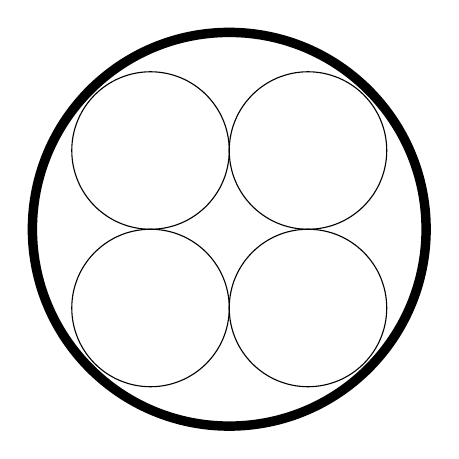
\begin{tikzpicture}
        \draw [line width=1.2mm] (0,0) circle (2.5) ;
        \draw (1,1) circle (1);
        \draw (-1,1) circle (1);
        \draw (-1,-1) circle (1);
        \draw (1,-1) circle (1);
    \end{tikzpicture}
    \caption{Fiber Model}
    \label{fig:fiber}
\end{figure}

\subsection{Modeling Behavior of \ch{Ag+} ions}
We model the fiber as shown in Figure \ref{fig:fiber}. We assume that the \ch{Ag+} ions diffuse into the fiber and fit in-between the polyurethane strands. Ignoring the effects of the strands, we can approximate the fiber as a structure similar to a capillary (an open area surrounded by a membrane).

Assume that the fiber is a cylinder of radius $r$ of $100\mu m$ and a length $2L$ of $3cm$. Assume also that the fiber is fully saturated with a solution of 35\% wt \ch{Ag} precursor, and taking the diffusion coefficent of silver to be $1.5 \times 10^{-5}cm^{2}s^{-1}$~\cite{diff_silver}. 

\begin{table}[ht]
    \centering
    \begin{tabular}{lcc}
    \hline
    Quantity && Value \\
    \hline
    Fiber half-length, \textit{L} && $1.5*10^{-2}m$ \\
    Fiber radius (initial), \textit{a} && $100 * 10^{-6}m$ \\
    Fiber radius (final), \textit{r} && $132 * 10^{-6}m$ \\
    Aqueous diffusivity of \ch{Ag}, $D_a$ &&  $1.5 \times 10^{-9}m^{2}s^{-1}$\\
    \end{tabular}
    \caption{Parameter Values for Fiber}
    \label{tab:my_label}
\end{table}
 
Assuming the absorption of the silver swells the fibre to 73\% of the original value~\cite{cond_shell}, we find the new radius to be $r*(1 + \sqrt{1.73}) = 132\mu m$.

%Hence the volume of the fiber will be: \begin{equation*}
%   {V = \pi r^{2}2L}
%\end{equation*}
%Hence we find the volume $V \approx 1.64 \times 10^{-9}m^3$

Using the model for capillary permeability used by Daniels et al~\cite{capillary_diffusion} (ignoring radial diffusion as the fiber is very thin and diffusion across the membrane), we find the Process time $t_p$ for the concentration to fall to $e^{-1}$ of its initial value to be $t_p = r/2k_m$, where $k_m$ is the permeability of the membrane.

\begin{figure}[ht]
    \centering
    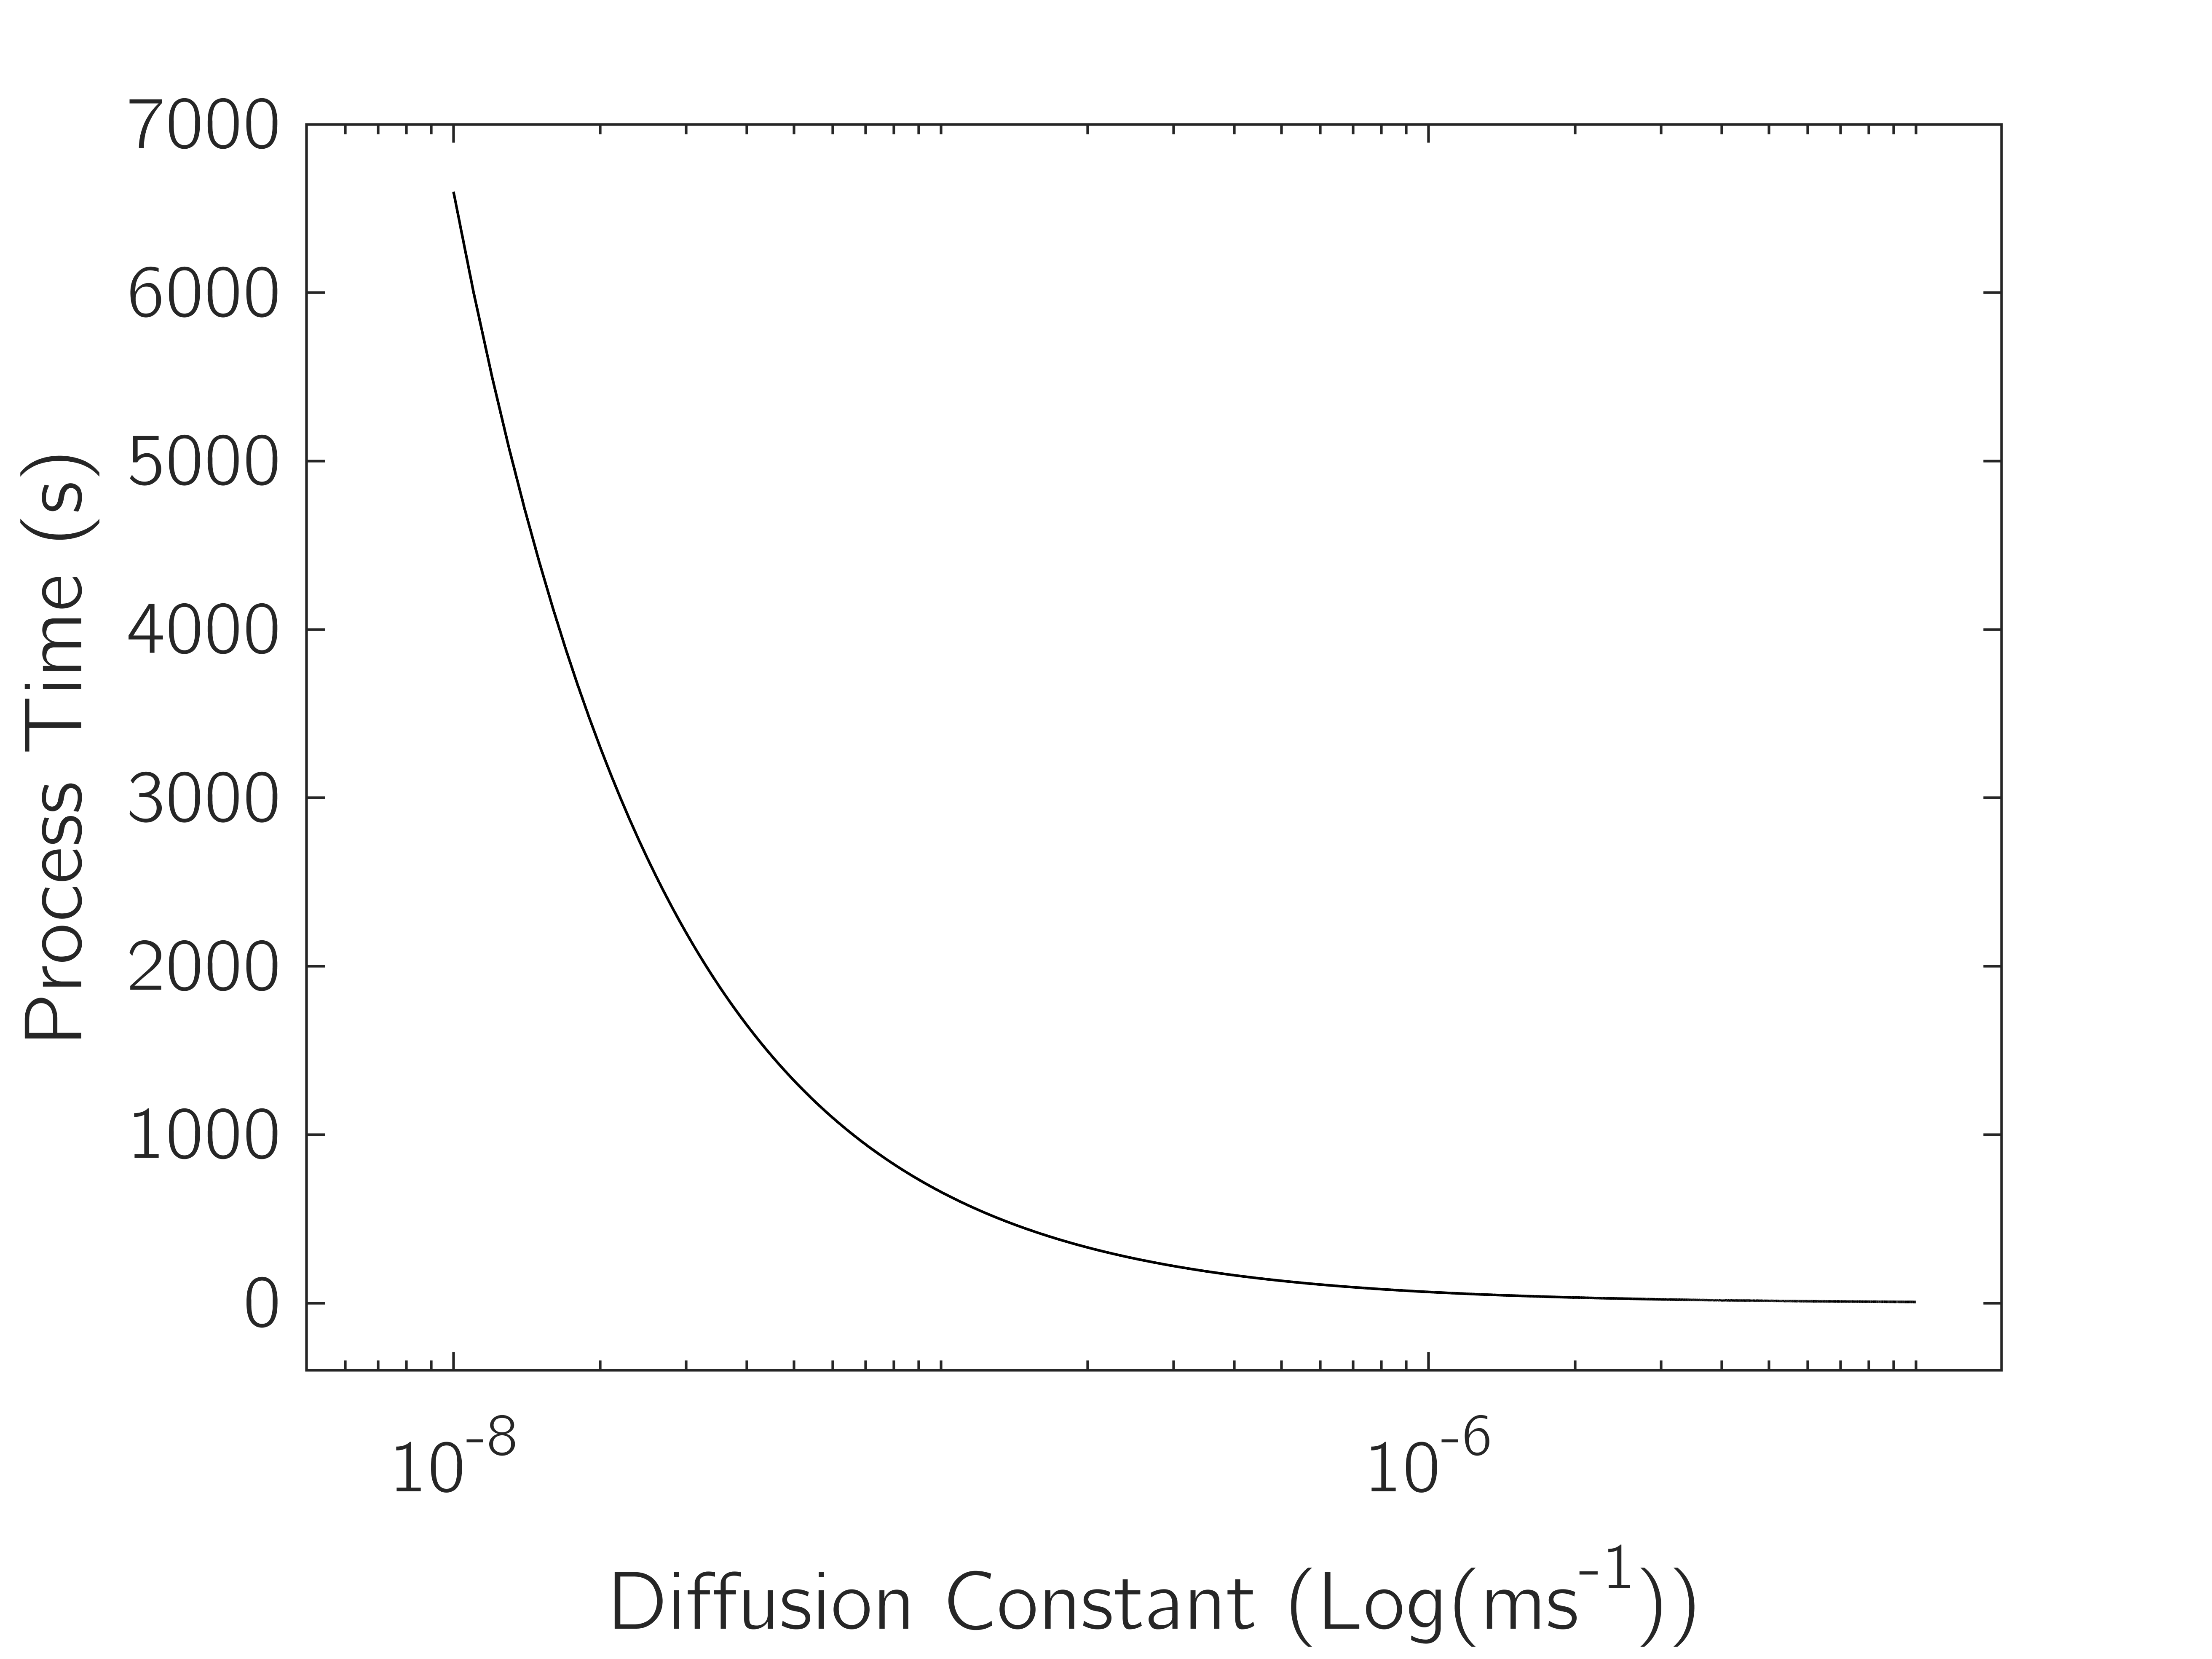
\includegraphics[width=.6\textwidth, keepaspectratio]{figures/diff_time.png}
    \caption{Effect of Permeability on Process Time}
    \label{perm_process}
\end{figure}

As the permeability of the finishing agent is not known, we plot the process time $t_p$ against a range of permeability as shown in Figure \ref{perm_process}. We note that for the process time of silver to be in the hours ($t_p > 3600s$) the membrane must have a permeability on the order of $10^{-7}$ to $10^{-8}$.

\pagebreak
\subsection{Comparison of Reducing Agents}
The two reducing agents are shown in Figure \ref{reducing_agents}. We note that hydrazine is a much smaller molecule than ascorbic acid~\cite{size_hydrazine,size_ascorbic} which means that it should diffuse faster. Furthermore hydrazine is a stronger reducing agent compared to ascorbic acid~\cite{kinetics_hydrazine,kinetics_ascorbic}.
These two factors meant that the proportion of silver particles inside the fiber is likely to be higher when hydrazine hydrate is used as reducing agent, as hydrazine will be able to diffuse into the fiber with greater ease, and will be better at reducing the \ch{Ag+} ions.

\begin{figure}[ht]
    \centering
    \subfloat[Hydrazine]
    {{\chemfig{N(-[3]H)(-[5]H)-N(-[1]H)-[7]H}}}%
    \qquad
    \subfloat[Ascorbic Acid]
    {{\chemfig{[:20]*5((-HO)=(-OH)-(=O)-O-(-(<:[:95]OH)-[:-150](-[:135]HO))(<:[:95]H)-)}}}%
    \caption{Reducing Agents}%
    \label{reducing_agents}%
\end{figure}

A third factor could be related to the finishing agent. In the original process, the reducing solution was a mixture of hydrazine hydrate and ethanol (1:1 volume ratio). In the new process the solution was an aqueous solution of ascorbic acid. If the permeability of the fiber to ethanol is greater than that of water, then the hydrazine will more readily diffuse in.

A final point is that the \ch{OH} groups in ascorbic acid have the potential to form hydrogen bonds with polyurethane. This may result in the ascorbic acid molecules "sticking" to the strands of the polyurethane, impeding the reduction process.

\section{Single Cycle}
In single cycle tests we found the results of the experiments to be unreliable. In many cases, three fibers would display very different resistances under the same conditions. Furthermore the fibers were extremely sensitive to strain, with small strains resulting in the fibers becoming non-conducting. However, we can notice some general trends, and some examples of typical experiments are included below.
\subsection{Effect of Concentration}
In the experiment shown in Figure \ref{single_resistance_conc}, three \textit{Ascorbic Acid Concentrations} of 0.0032 wt, 0.008 wt, and 0.016 wt were used for a \textit{Single Cycle} of immersion-reduction, with a 2 hour \textit{Ascorbic Acid Immersion Time}.

\begin{figure}[ht]
    \centering
    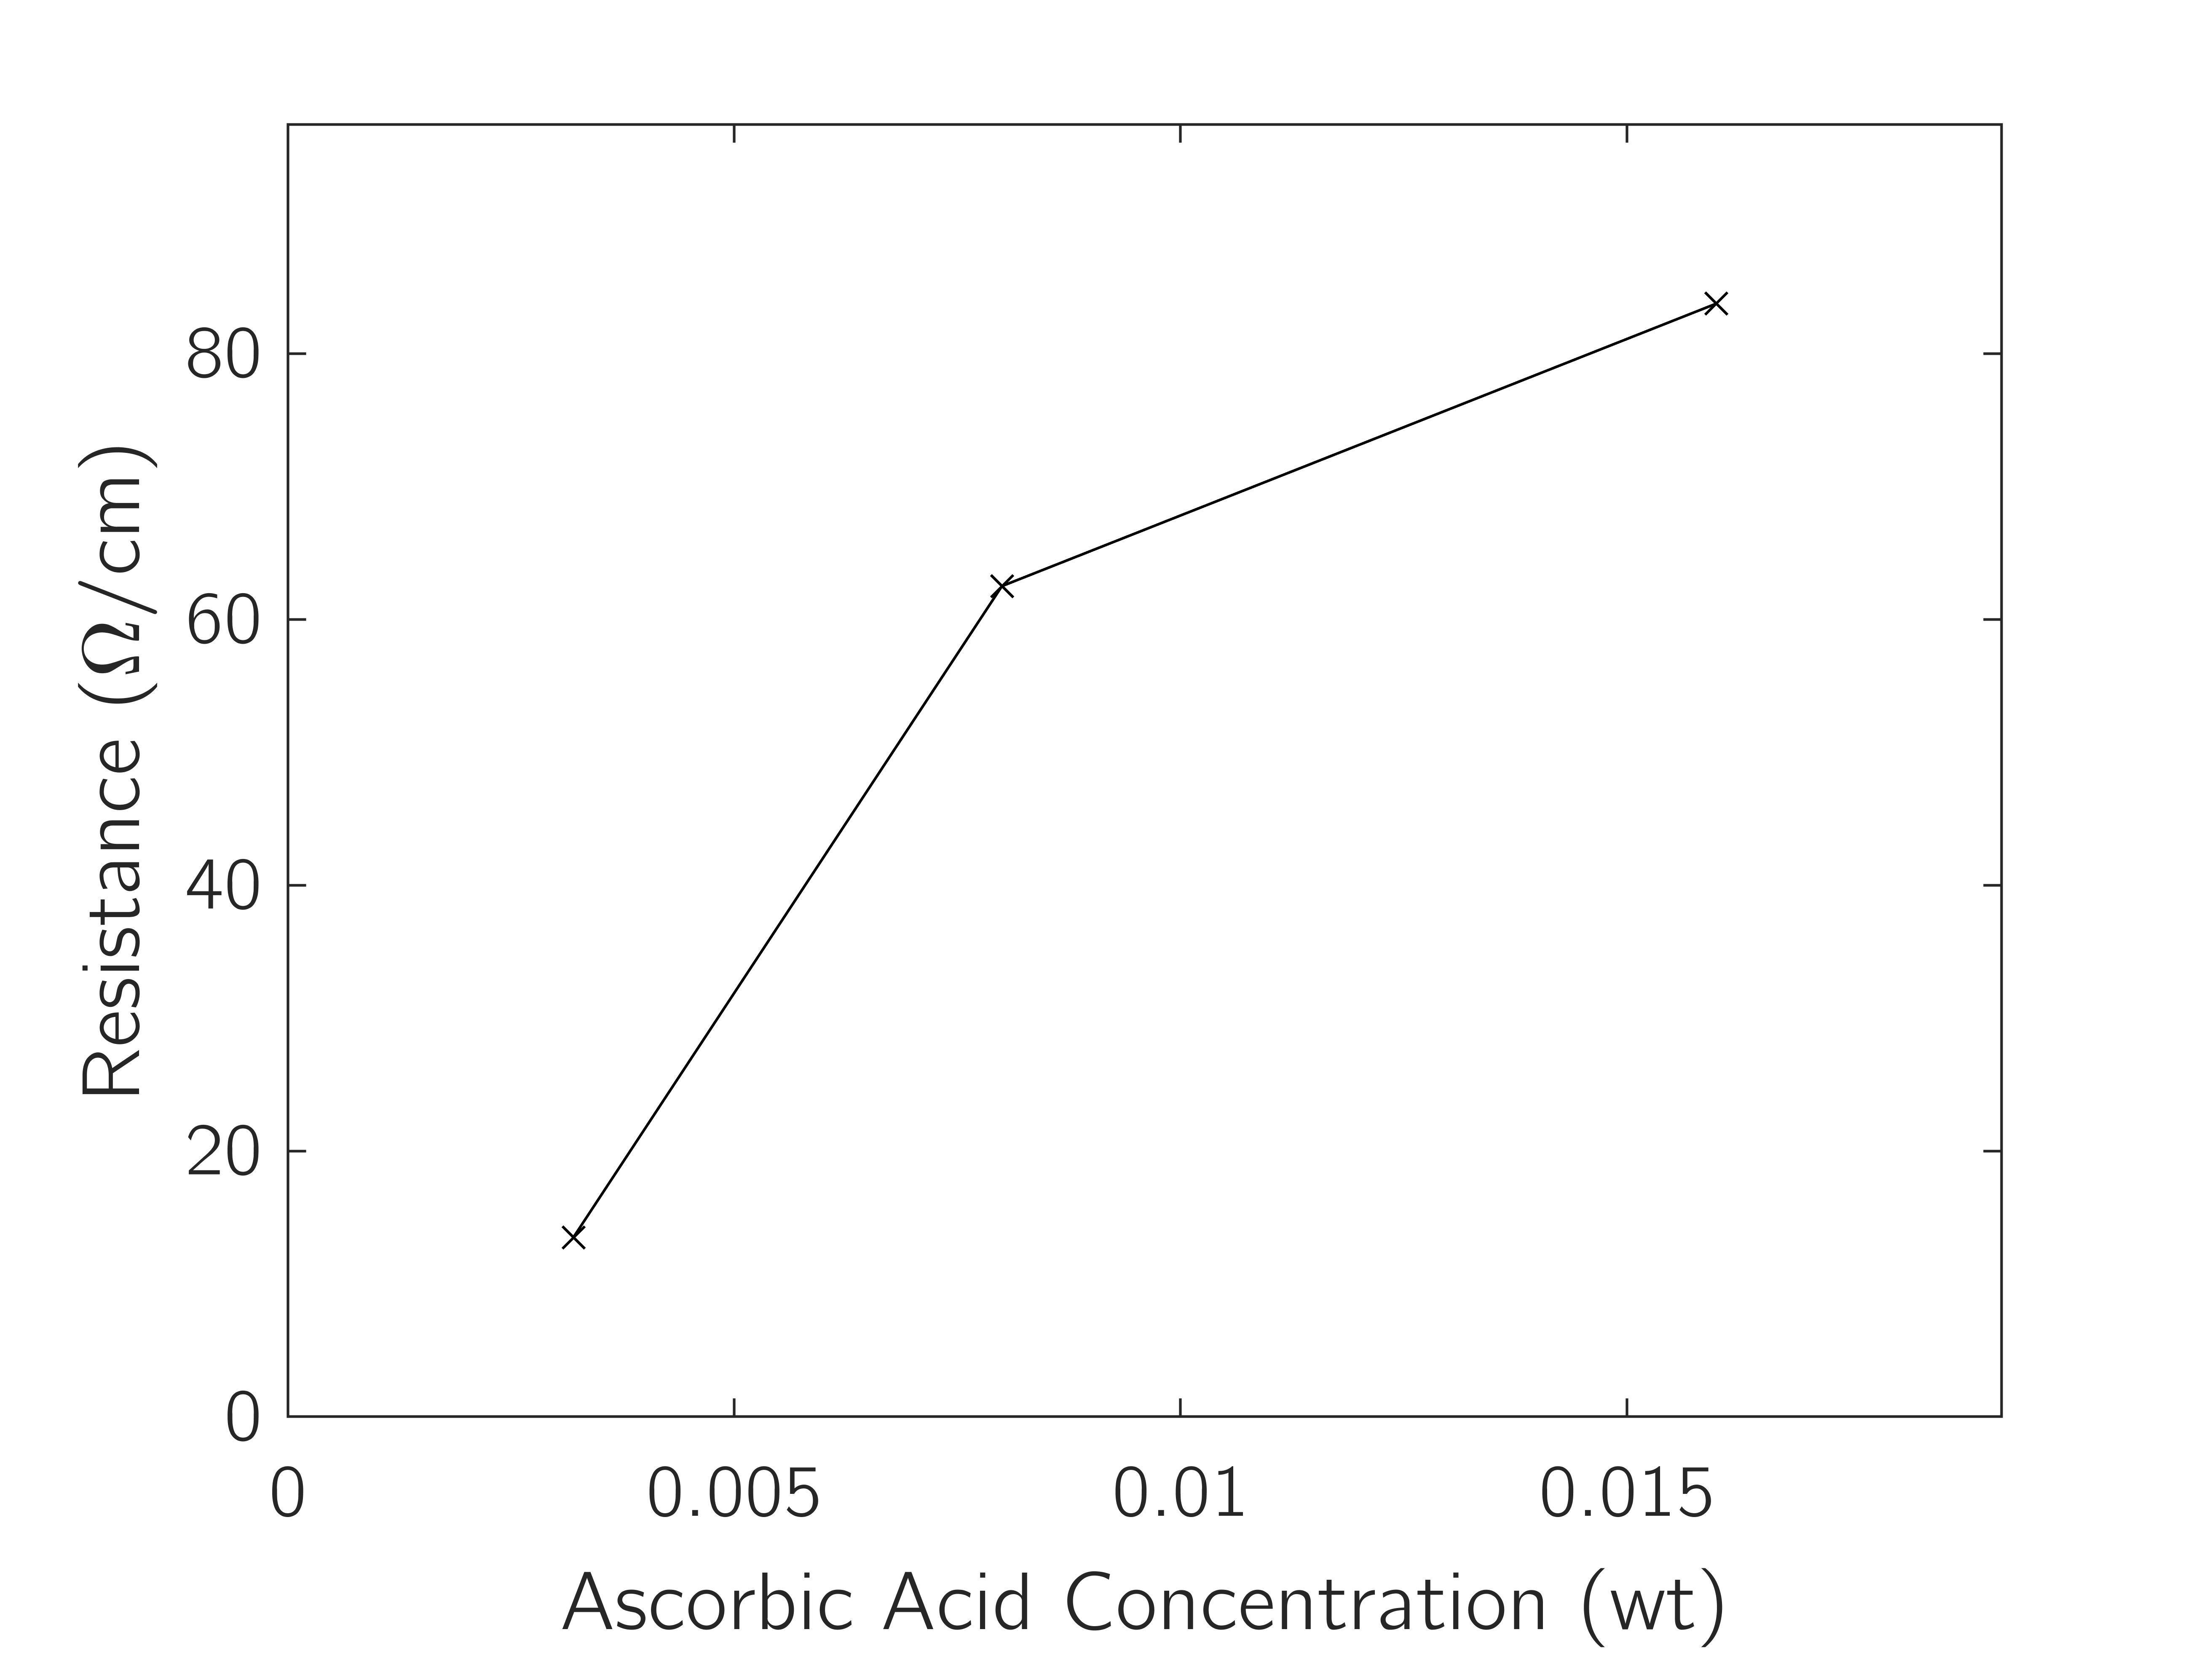
\includegraphics[width=.6\textwidth, keepaspectratio]{figures/single_resistance_concentration.png}
    \caption{Effect of Ascorbic Acid Concentration on Resistance}
    \label{single_resistance_conc}
\end{figure}
In Figure \ref{single_resistance_conc} the lower concentrations of Ascorbic Acid display lower average resistances than higher concentrations, and as rule this trend held. This is a non-intuitive result: it is expected that a higher concentration would lead to a faster reaction, meaning more \ch{Ag} particles inside the fiber, and hence higher conductivity. 
\\This is not the case, which leads us to hypothesise that ascorbic acid has difficulty entering the fiber. Hence a high concentration would mean a faster reaction near the edge of fiber, which would result in a higher concentration gradient for \ch{Ag+} ions from the centre to the edge, and hence faster diffusion of the \ch{Ag+} ions out of the core, resulting in less \ch{Ag} nanoparticles within the fiber.

\subsection{Effect of Time}
In the experiment shown in Figure \ref{single_resistance_time}, a single \textit{Ascorbic Acid Concentrations} of 0.0032 wt was used for a \textit{Single Cycle} of immersion-reduction, with  1, 2, and 3 hour \textit{Ascorbic Acid Immersion Times}. 

\begin{figure}[ht]
    \centering
    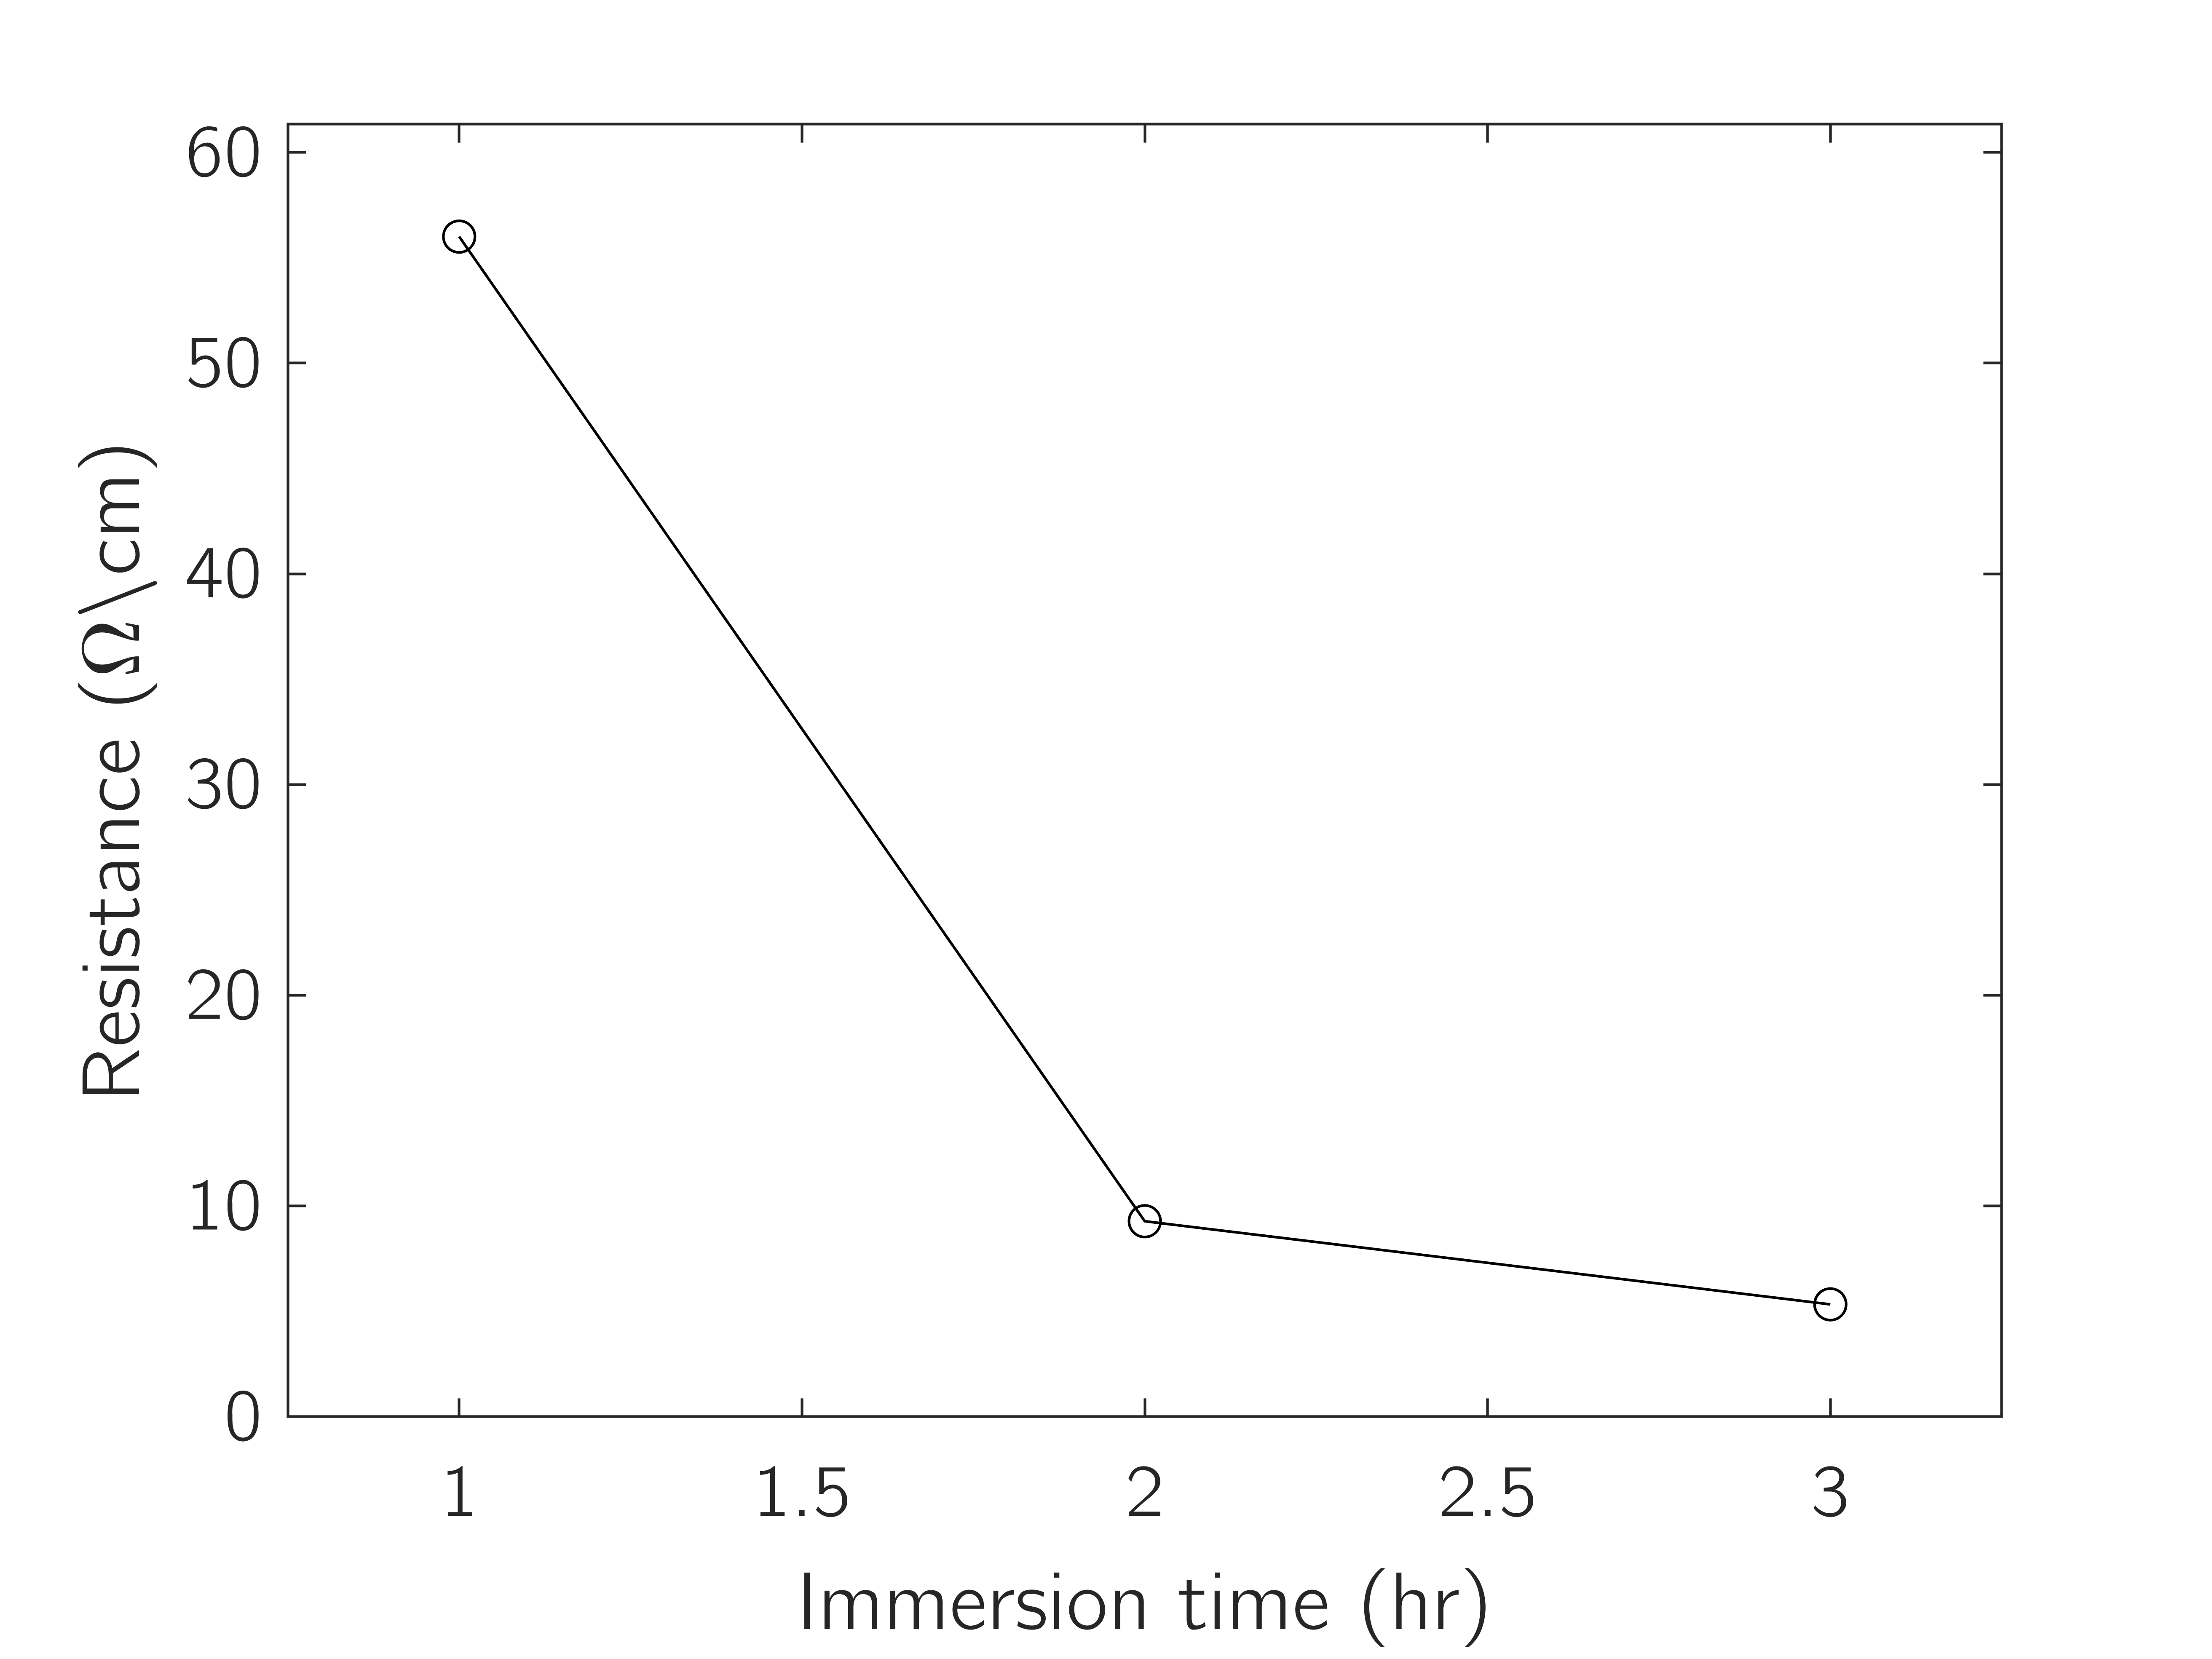
\includegraphics[width=.6\textwidth, keepaspectratio]{figures/single_resistance_time.png}
    \caption{Effect of Immersion Time on Resistance}
    \label{single_resistance_time}
\end{figure}

In Figure \ref{single_resistance_time} with increased time there was a lower average resistance. Hence we deduce that with longer time, a higher proportion of \ch{Ag+} ions will be reduced, leading to more \ch{Ag} nanoparticles and higher conductivity.

\pagebreak
\section{Multi-cycle Reduction}
Here the fibers underwent multiple immersion reduction cycles. Each re-immersion in the precursor
re-saturates the fiber with \ch{Ag+} ions. 
Hence the total number of \ch{Ag} nanoparticles is expected to be much higher at the end of four cycles as compared to a single cycle.

\subsection{Effect of Concentration}
In the experiment shown in Figure \ref{multi_resistance_concentration}, the \textit{Ascorbic Acid Immersion Time} was held constant at one hour, with \textit{Four Cycles} of immersion-reduction. The \textit{Ascorbic Acid Concentrations} were varied from 0.004 wt to 0.032 wt. There were a total of three samples for each cycle/concentration (48 samples in total). \\In the first immersion-reduction cycle, none of the samples reduced by 0.008 wt were conducting---hence the lack of a data-point. With that exception, it is interesting to note that the samples follow the trend described in Section 3.1.1 with lower concentrations having a lower average resistance.

\begin{figure}[ht]
    \centering
    \subfloat[Full Graph]
    {{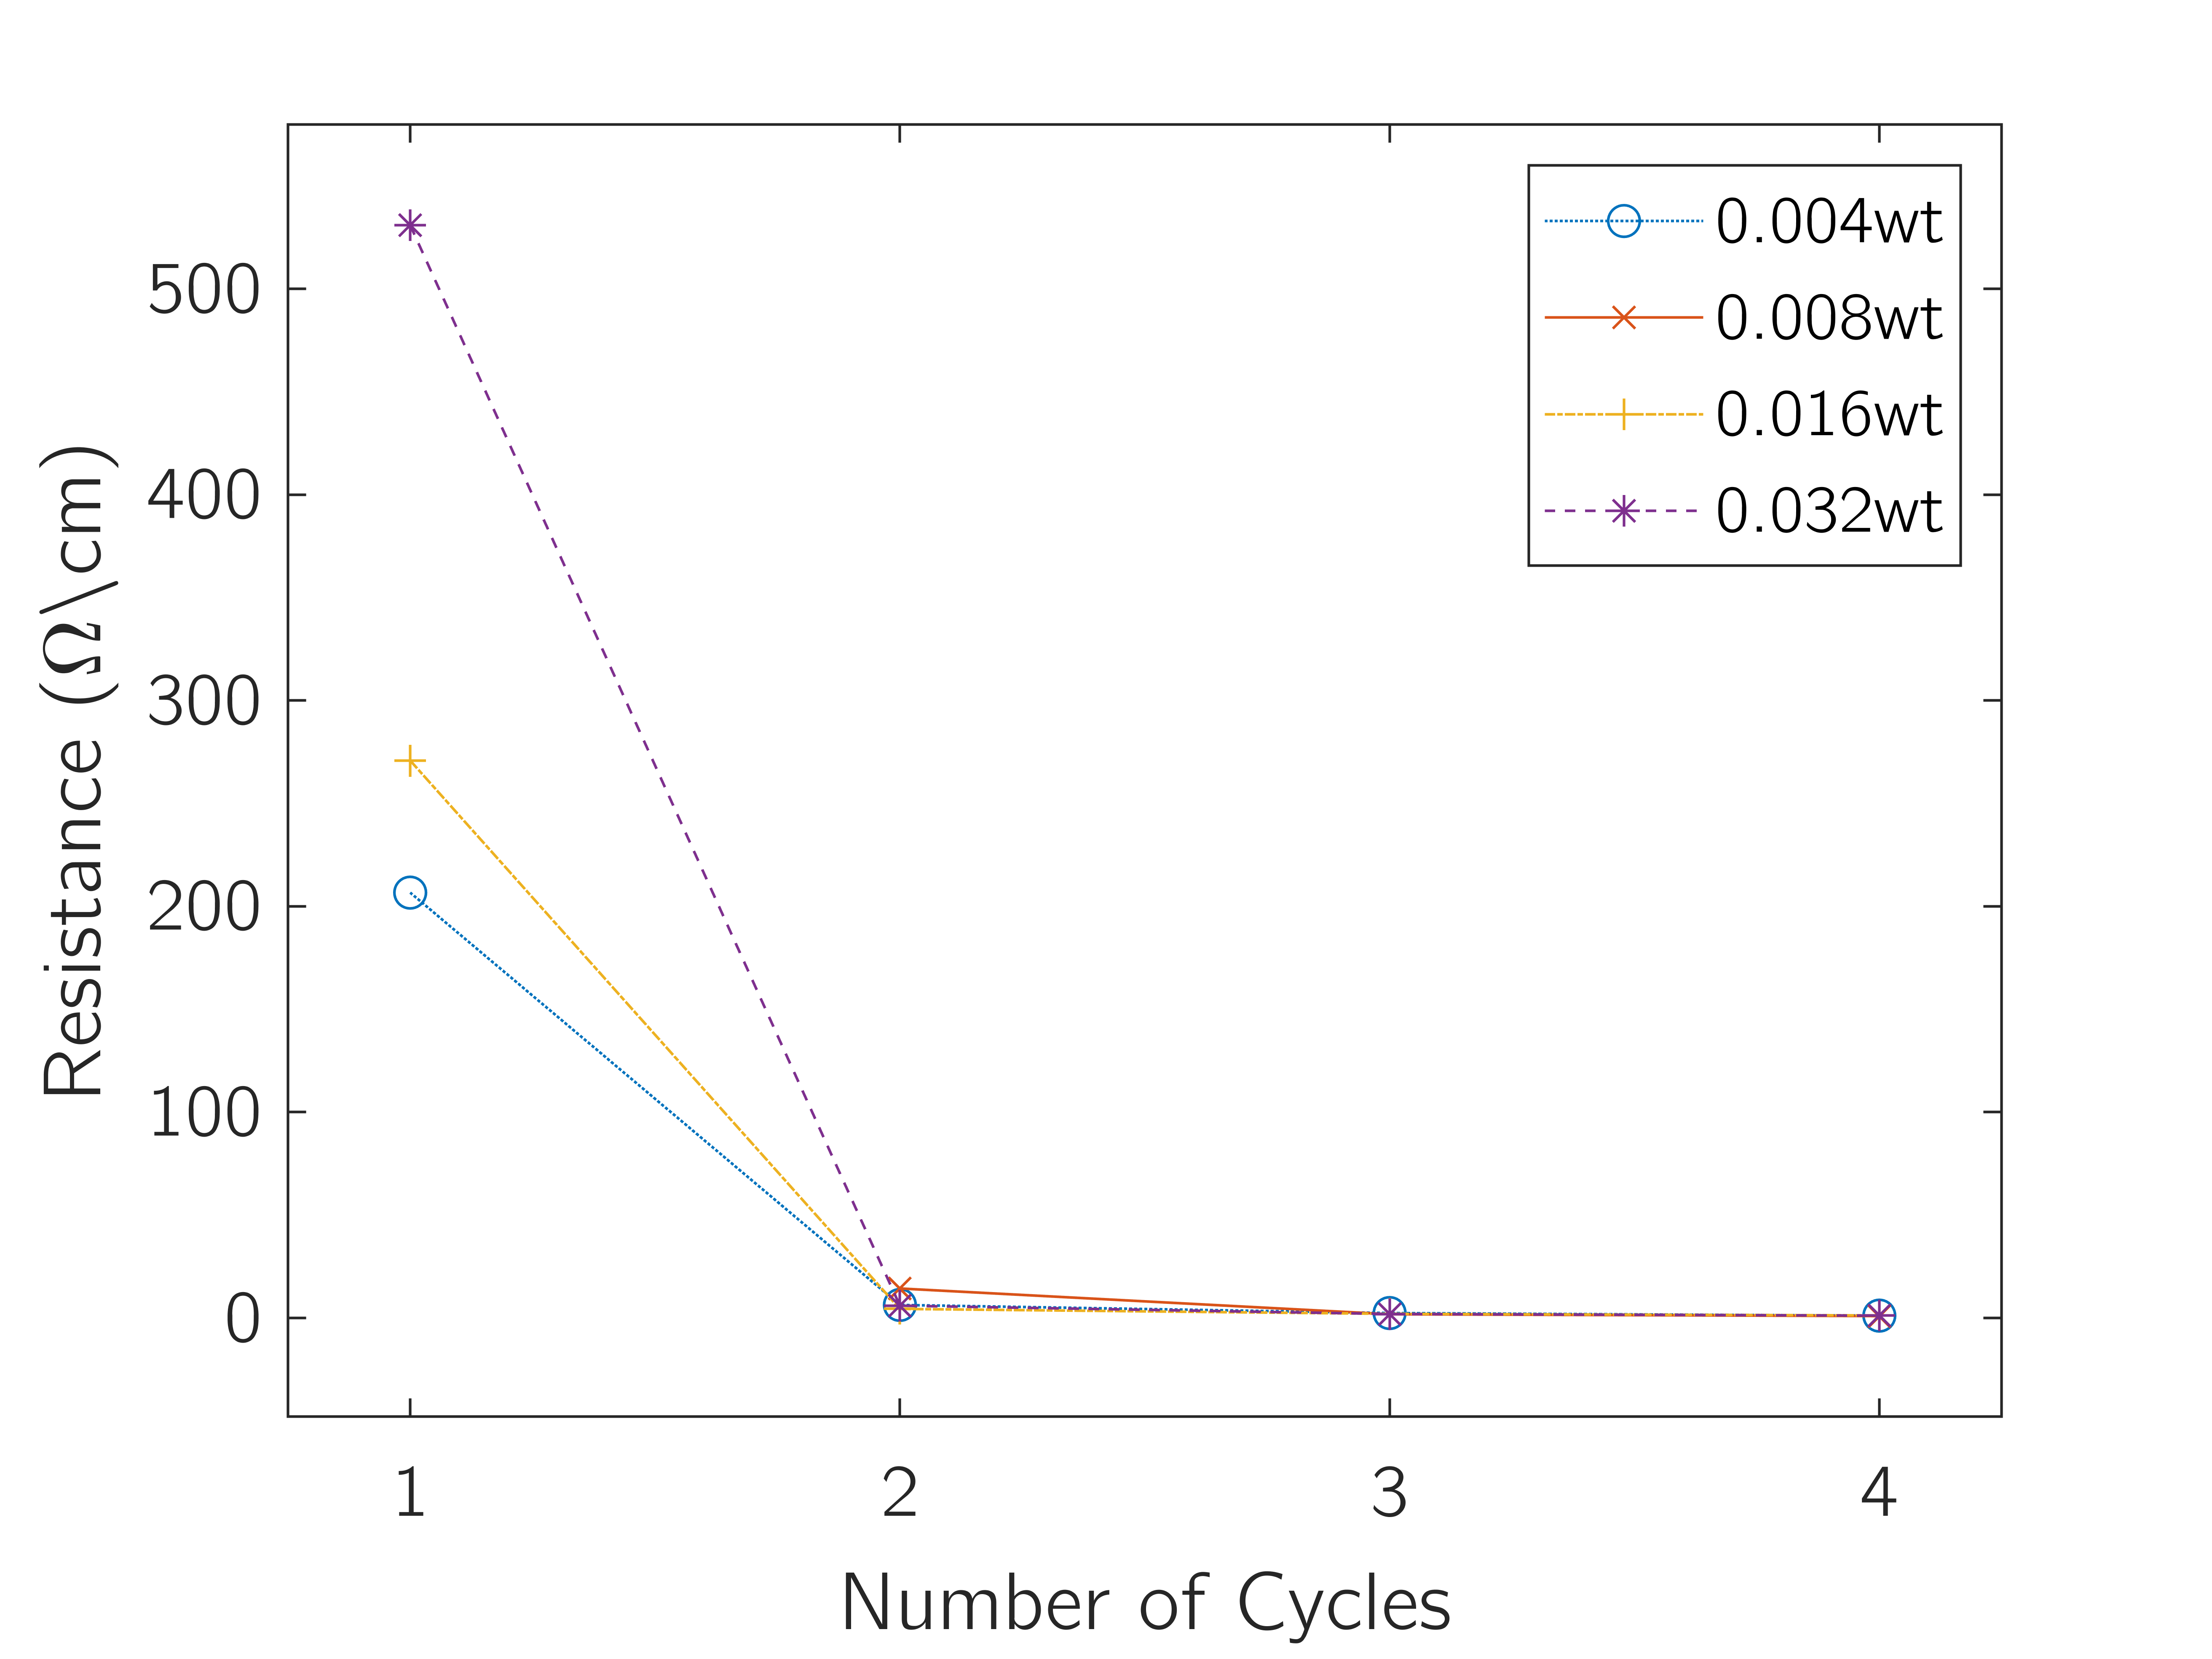
\includegraphics[width=.45\textwidth]{figures/multi_resistance_concentration.png} }}%
    \qquad
    \subfloat[Zoomed]
    {{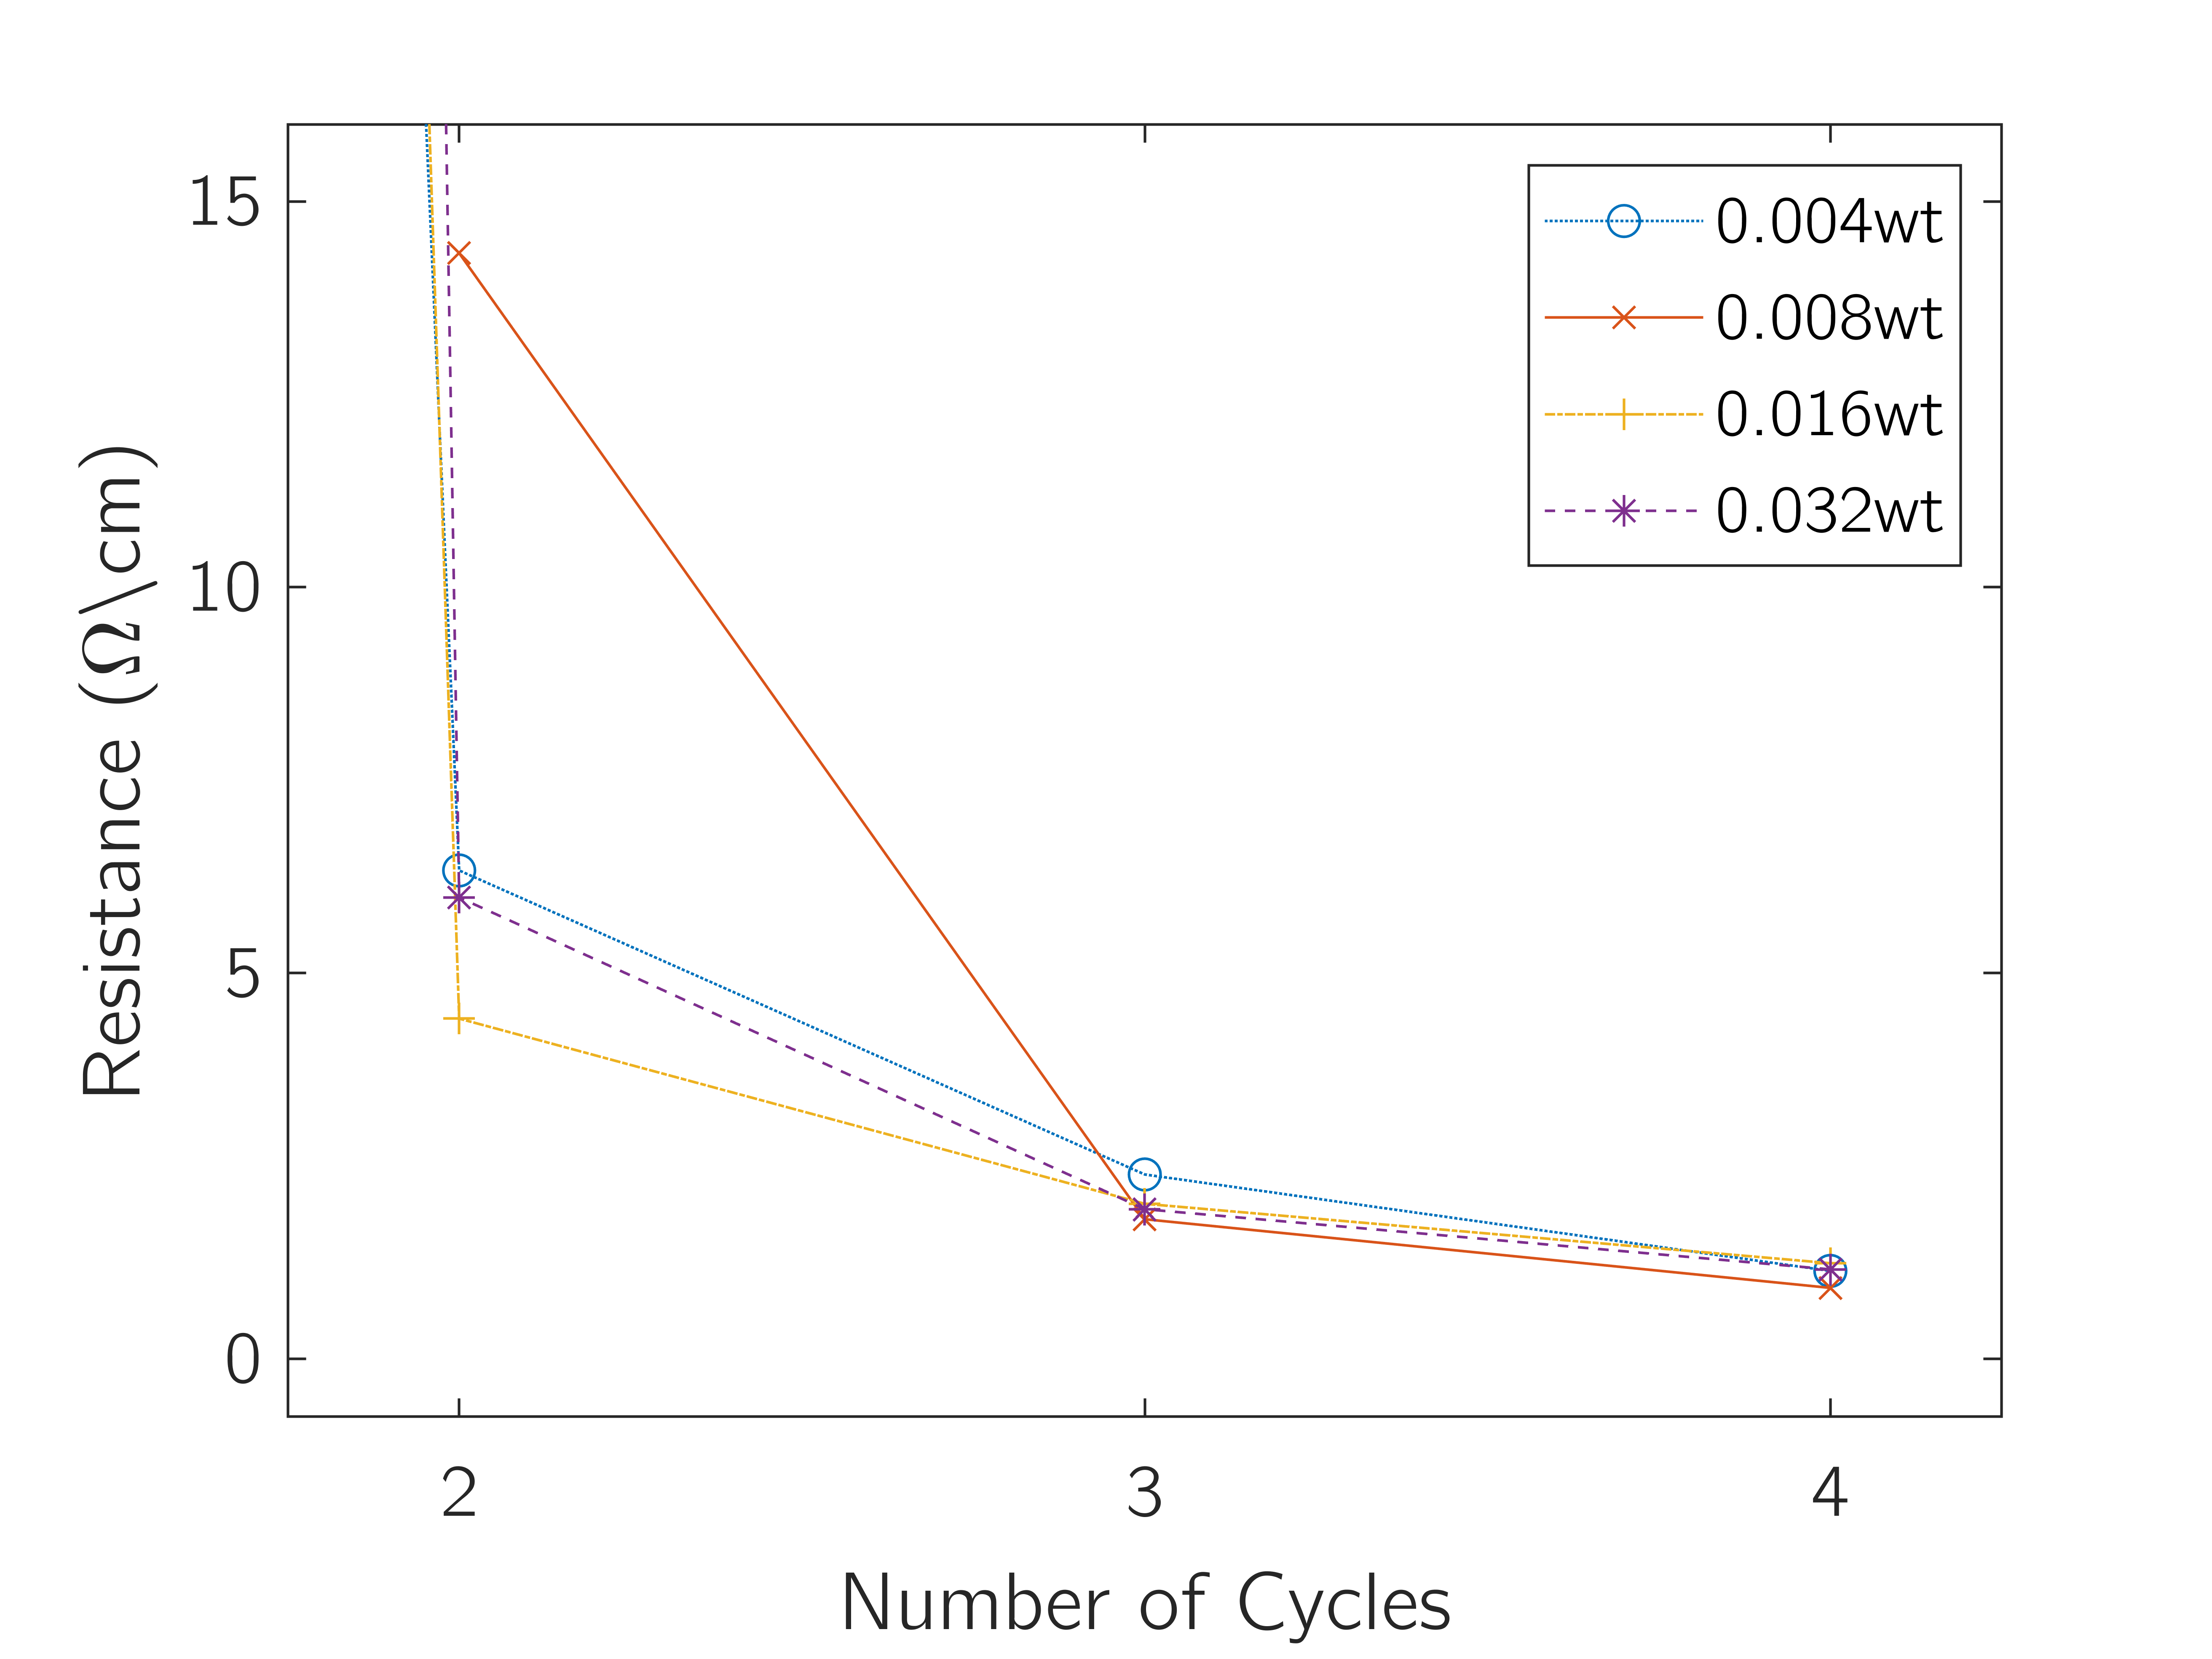
\includegraphics[width=.45\textwidth]{figures/multi_resistance_concentration_zoomed.png} }}%
    \caption{Effect of Concentration on Resistance}%
    \label{multi_resistance_concentration}%
\end{figure}

In Figure \ref{multi_resistance_concentration} we see that that beyond 2 cycles, the difference in the resistance quickly saturates. This implies the effect of concentration to resistance (Section 3.1.1) is noticeable at smaller densities of \ch{Ag} nanoparticles, but is a negligible effect at higher densities.


\pagebreak
\subsection{Effect of Time}
In the experiment shown in Figure \ref{fig:multi_resistance_time}, the \textit{Ascorbic Acid Concentration} was held constant at 0.016 wt with \textit{Four Cycles} of immersion-reduction. The \textit{Ascorbic Acid Immersion Time} was varied with times of 5, 15, 30 and 60 minutes. There were a total of three samples for each cycle/time (48 samples in total), but only the final resistances are displayed.

\begin{figure}[ht]
    \centering
    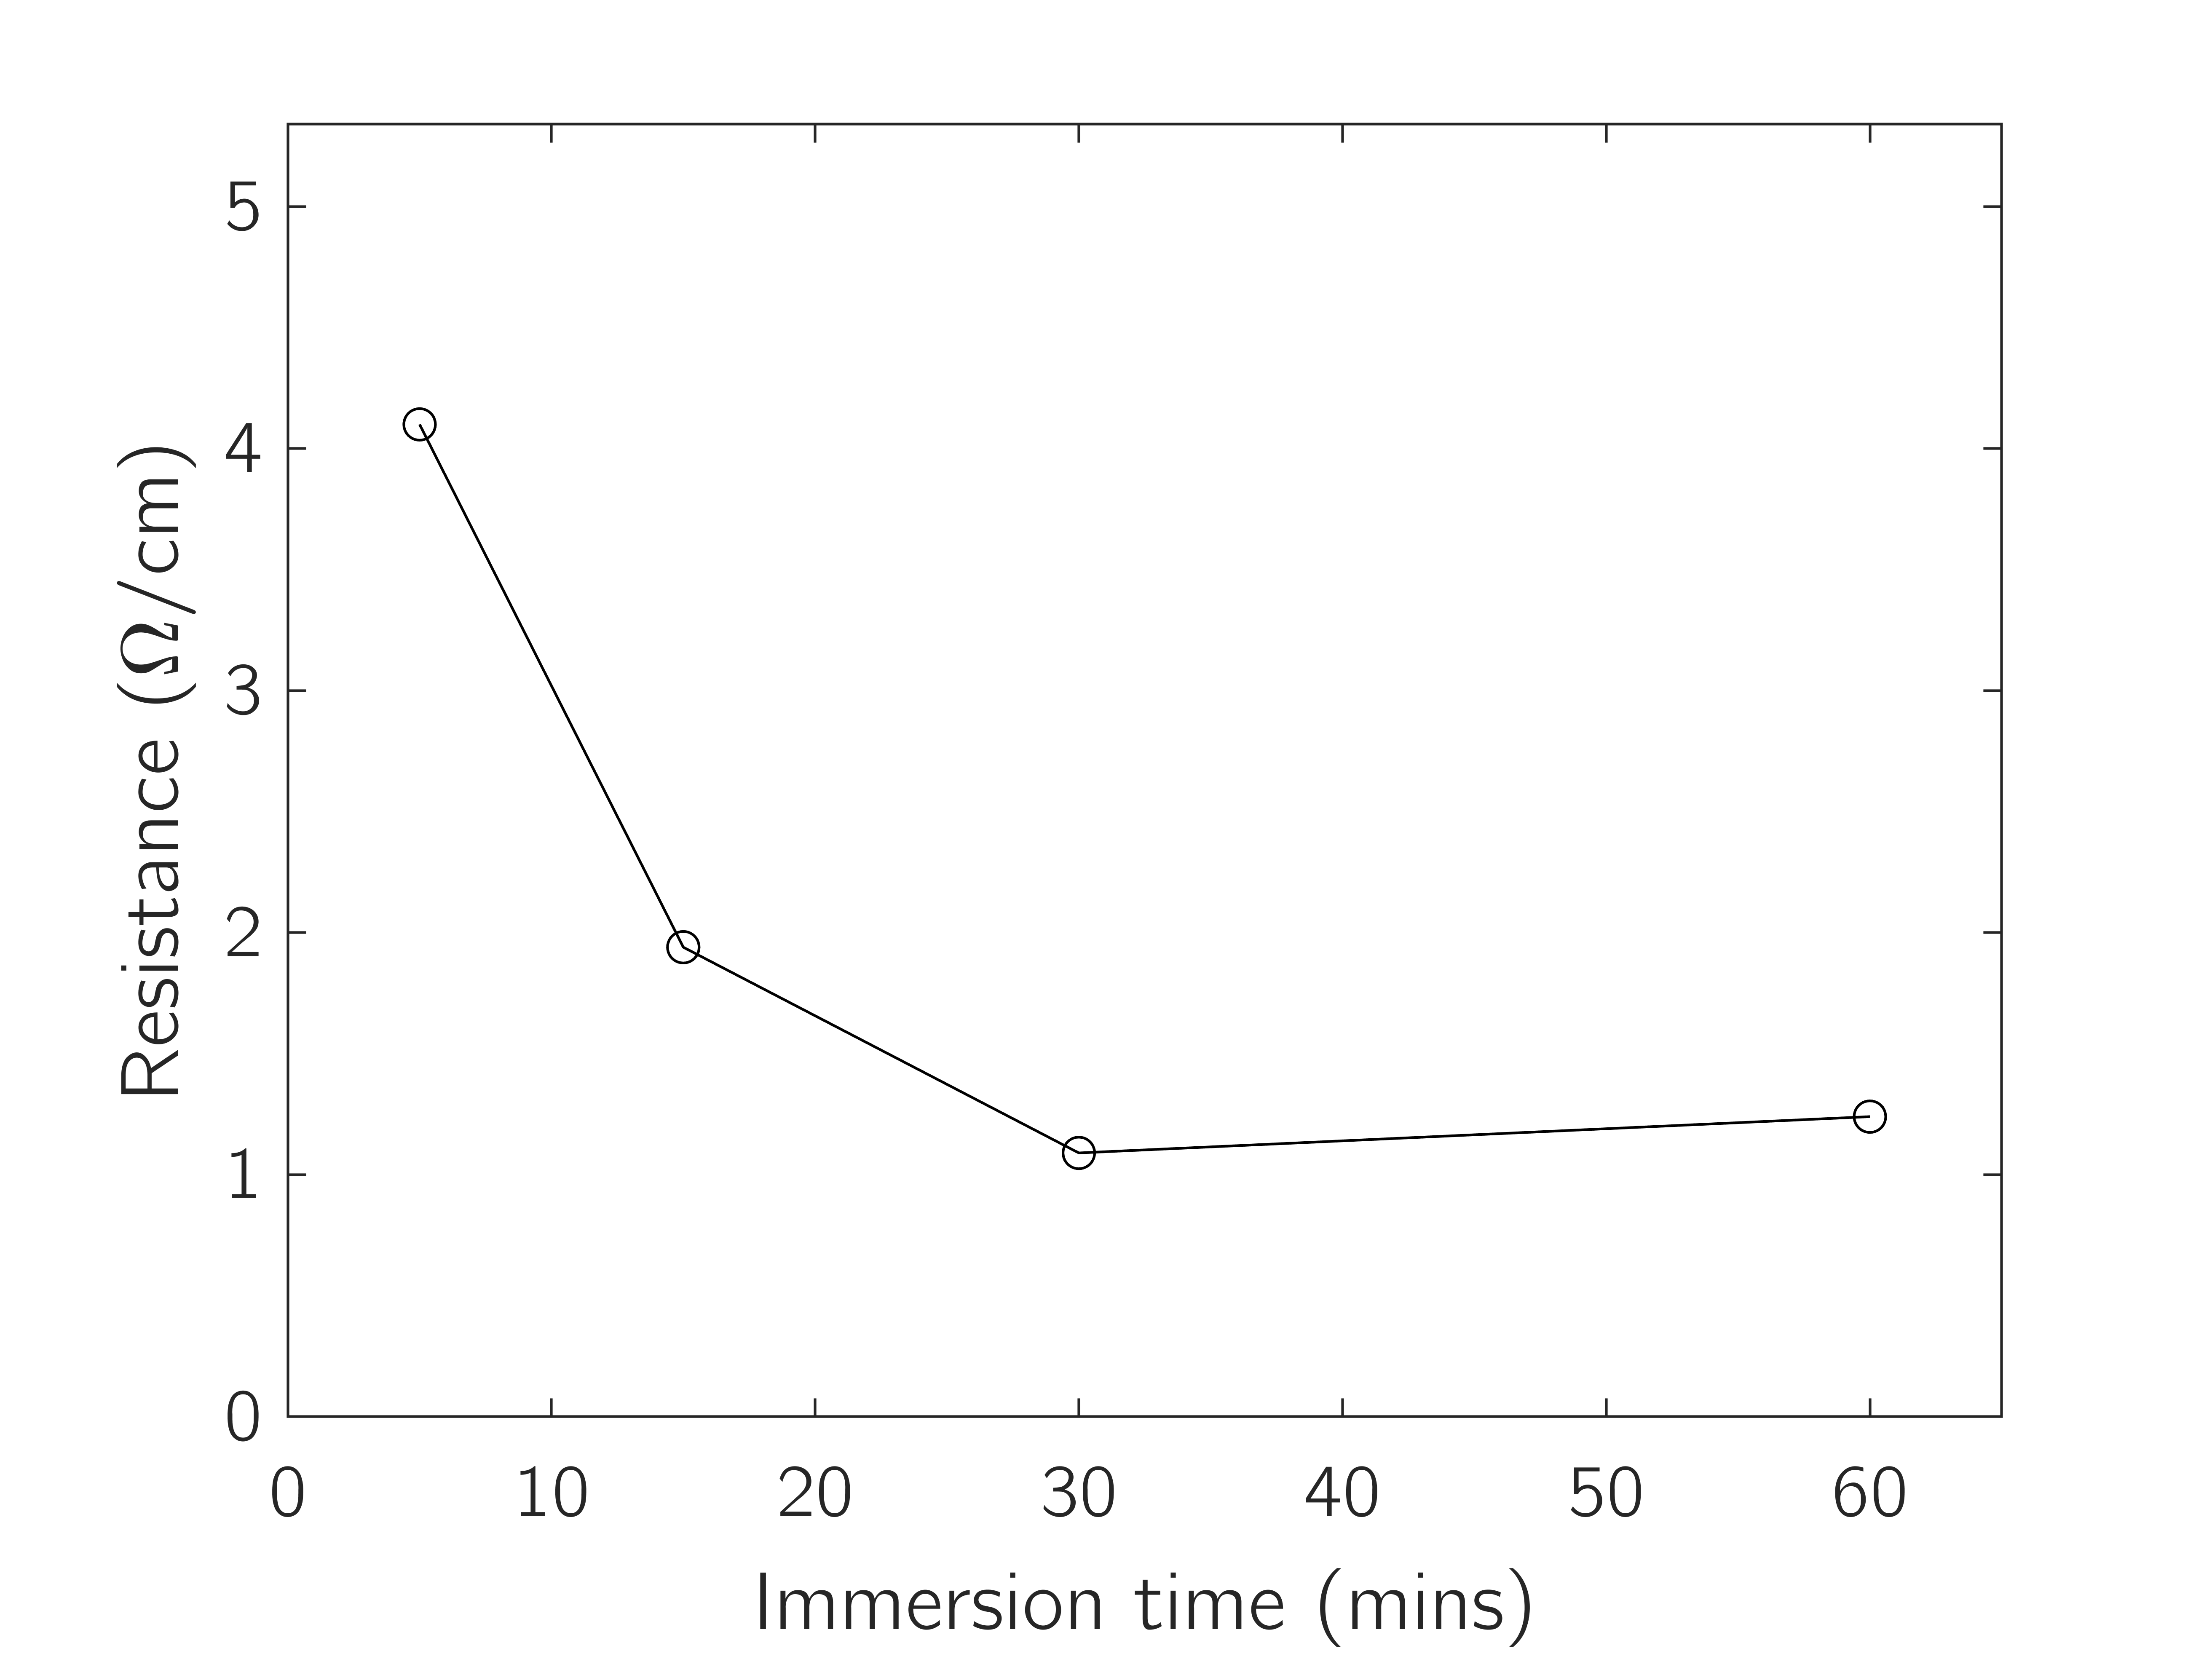
\includegraphics[width=0.6\columnwidth]{figures/multi_resistance_time.png}
    \caption{Effect of Immersion Time on Resistance}
    \label{fig:multi_resistance_time}
\end{figure}

In Figure \ref{fig:multi_resistance_time} we find that beyond a certain time ($\sim$ 30 mins), the effect of an increase in \textit{Ascorbic Acid Immersion Time} on conductivity is negligible. Hence we conclude that while some reduction may still be taking place (Section 3.1.2), the majority of the \ch{Ag+} ions are reduced in the first 30 minutes, and that, while the effect is noticeable in single cycles where the density of \ch{Ag+} ions is low, its effect is negligible at the higher densities of multiple cycles.

\section{Resistance-strain Behavior}
We are interested in the relationship between the resistance and the strain because the fibers are intended for use as strain sensors~\cite{jae2018} and hence the resistance/strain relationship should be characterised. Another reason for investigating the strain characteristic is that embedding \ch{Ag} particles into the fiber will change how the fiber responds to strain~\cite{cond_shell}.

\begin{figure}[ht]
    \centering
    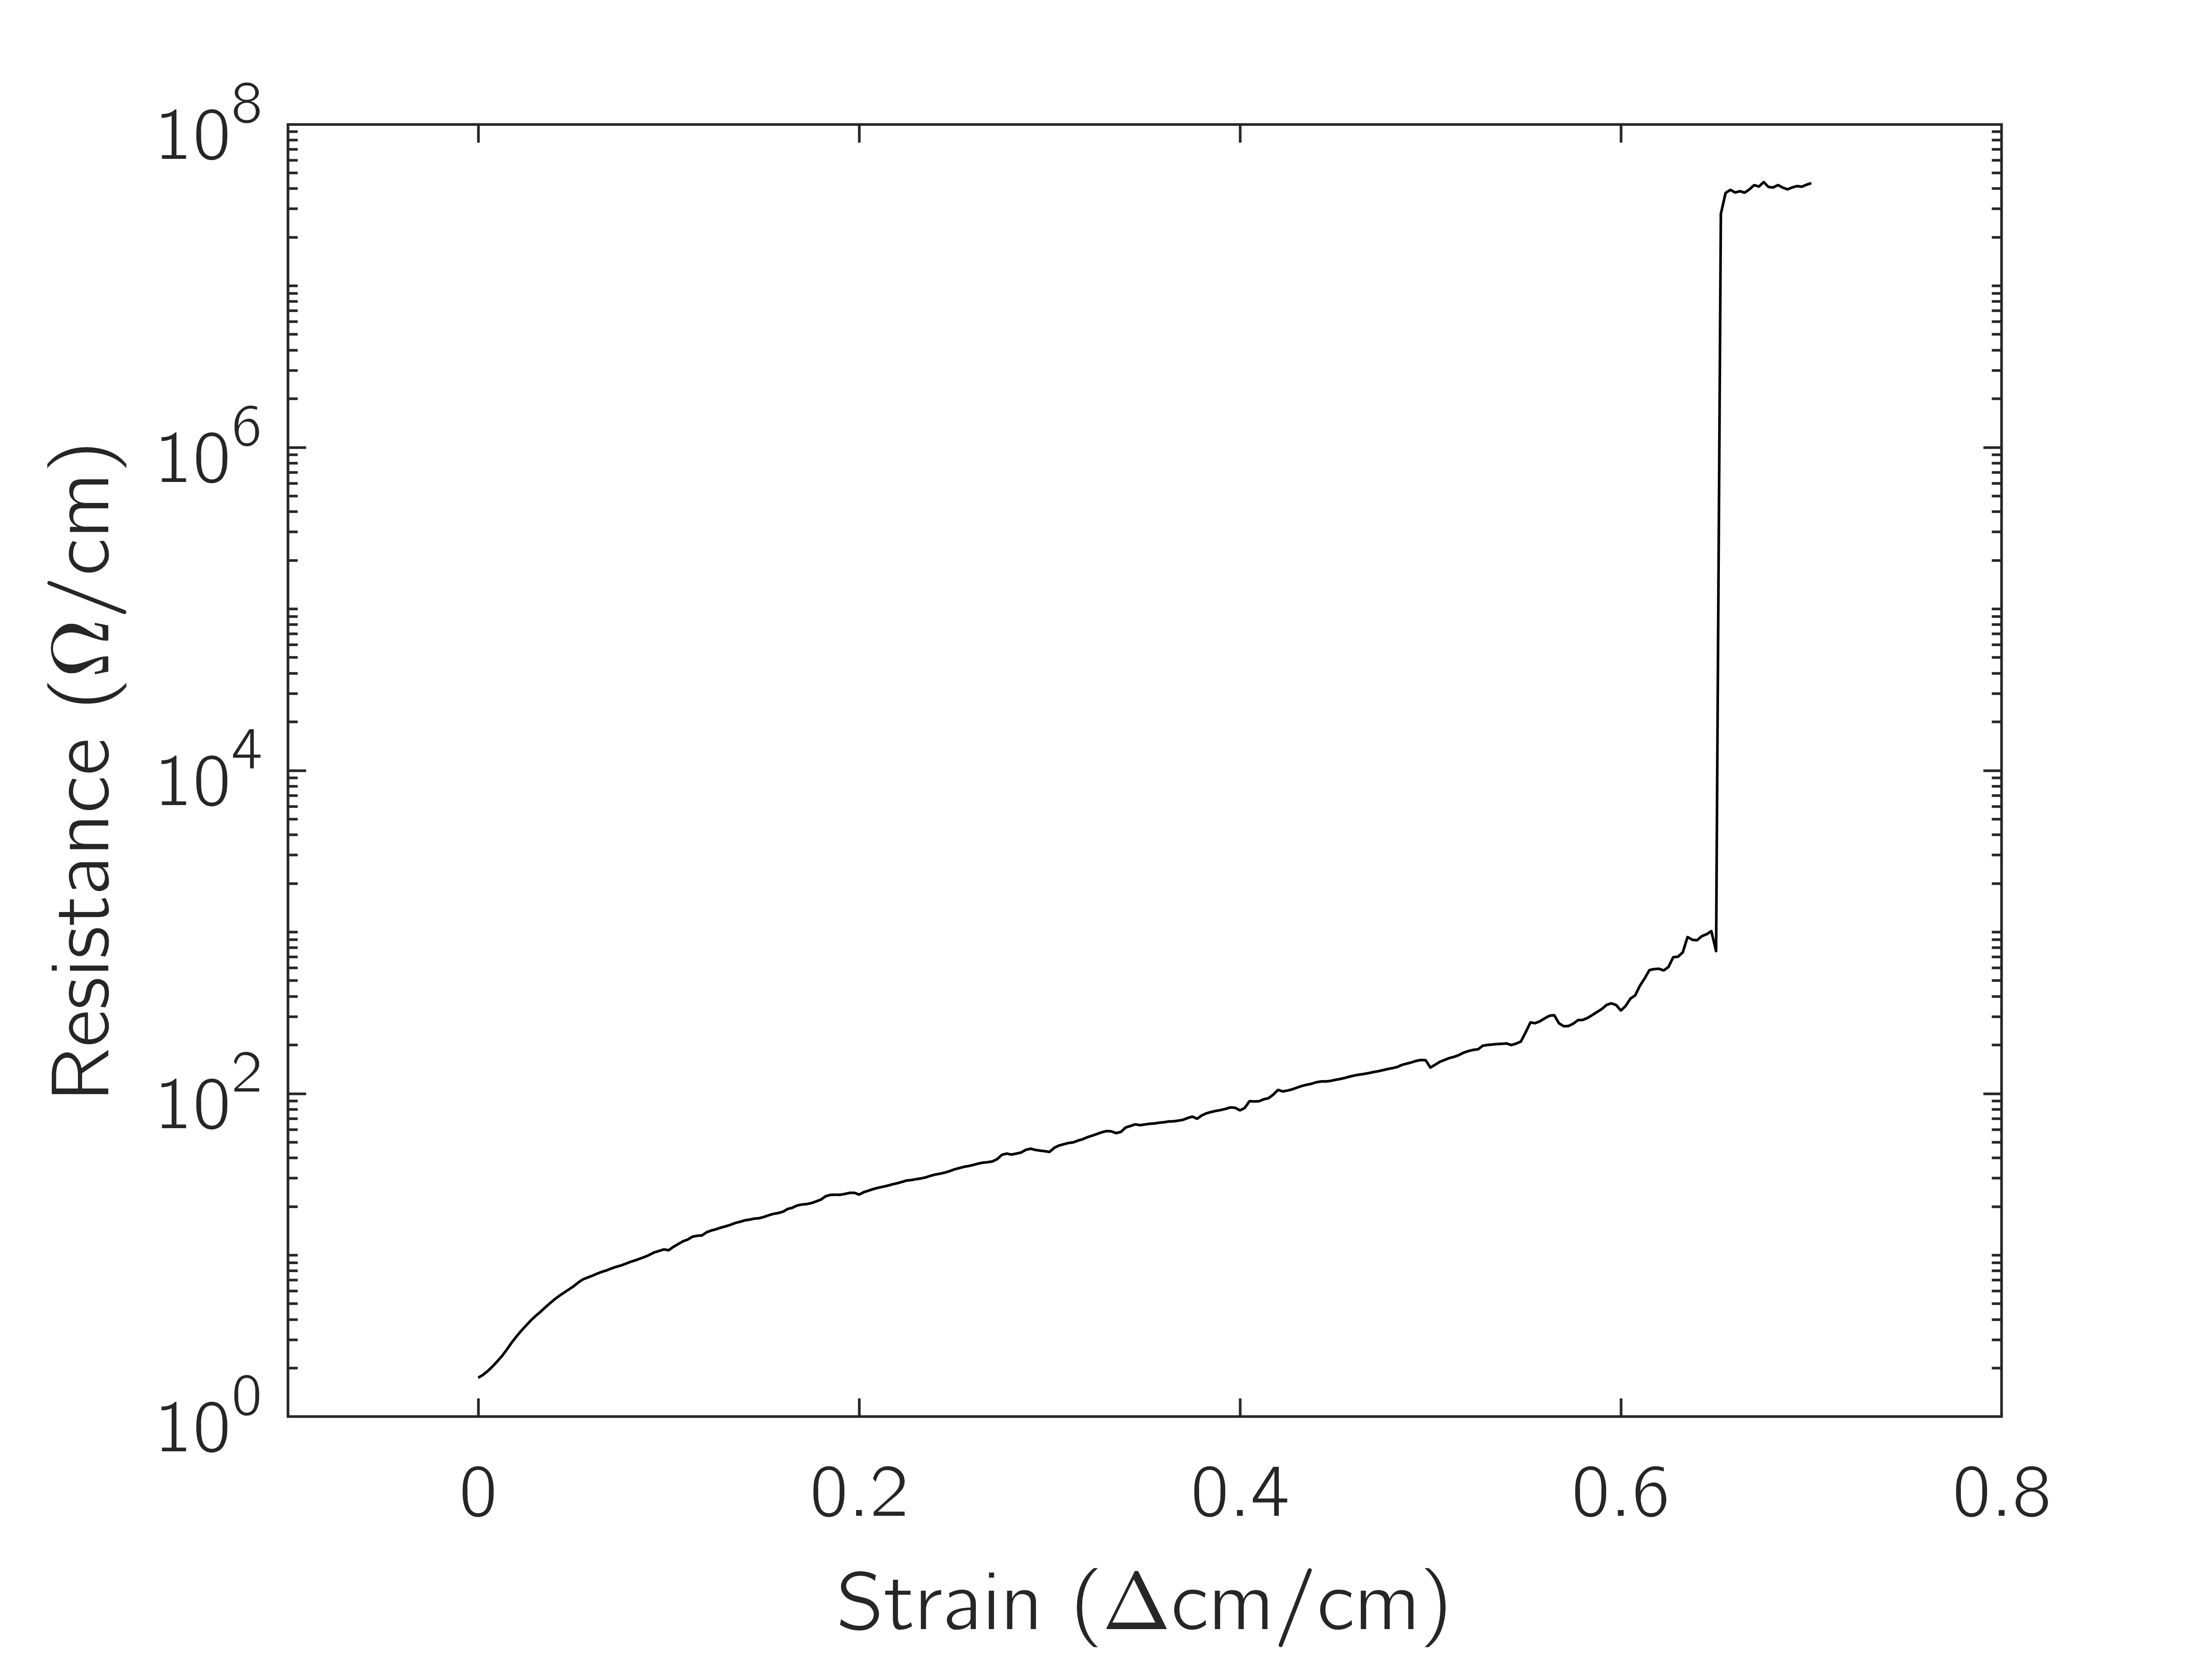
\includegraphics[width=0.7\columnwidth]{figures/strain_graph.png}
    \caption{Relationship of Strain and Resistance}
    \label{fig:strain_resistance}
\end{figure}

In Figure \ref{fig:strain_resistance} we see that the resistance of the fiber increases with increasing strain, until a point at $\sim 65\%$ where the fiber stops conducting and the resistance jumps to the $M\Omega$ range. This contrasts with the performance of the hydrazine reduced fibers, where conductivity is maintained until $\sim 340\%$ range~\cite{jae2018}.

The conductivity of the fiber comes from the contact of the \ch{Ag} nanoparticles embedded in the fiber with each other. As the fiber is stretched the proportion of \ch{Ag} nanoparticles in contact with each other is reduced. Hence the resistance of the fiber increases, until a point is reached where there is no contact between the \ch{Ag} nanoparticles and conductivity is lost~\cite{jae2018,cond_shell}. 

Furthermore, it has been seen that the \ch{Ag} shell at the surface of the breaks more easily, and hence at higher strains most of the conductivity comes from \ch{Ag} nanoparticles embedded inside the fiber~\cite{jae2018,cond_shell}. A possible explanation for the difference in the strain limit could be the size difference between the reducing agents. If ascorbic acid has difficulty diffusing in, then it is possible that the majority of the conductivity comes from \ch{Ag} nanoparticles on the outer layer of the fiber, hence the lower strain tolerance.

\chapter{Conclusion}
In summary we were able to fabricate highly stretchable conducting fibers by cyclically immersing spandex fibers in silver trifluoroacetate 
(\ch{AgCF3COO}) and ascorbic acid (\ch{C6H8O6}). 
The concentration of the silver trifluoroacetate was held at 35\% wt, while concentrations of 0.0032 - 0.032 wt were tested for the ascorbic acid, with no significant differences in performance for multiple cycles.

We found that the optimal method for producing conductive fibers was 4 cycles of immersion and reduction, with 30 minute immersion and reduction times. 

The resulting fibers had a resistance to the order of $10^0~\Omega cm^{-1}$ with the fibers conducting until a strain of $\sim 66\%$ strain. This is inferior to the fibers produced by the original process, where the fibers had a resistance to the order of $10^{-3}~\Omega cm^{-1}$ with the fibers conducting until a strain of $\sim 320\%$ strain~\cite{jae2018}.

We hypothesise that this is due to two reasons: First, because the kinetic properties of the hydrazine reaction are more favourable than those of the ascorbic acid reaction.~\cite{kinetics_hydrazine}, and second, because ascorbic acid is a larger molecule~\cite{size_ascorbic} than hydrazine hydrate~\cite{size_hydrazine}, and hence the diffusion of the reducing agent into the fiber may be slower in comparison, resulting in a lower concentration of \ch{Ag} nanoparticles inside the fiber.

However there is potential for improvement in the process. Control of temperature and PH~\cite{silver_size,temp_ascorb} has been shown to effect the size and quality of the \ch{Ag} nanoparticles. Another possible area for improvement involves the introduction of a catalyst or stabilising agent, both of which have been shown to improve the reaction speed of the ascorbic acid~\cite{ascorb_stabilising_agent, ascorb_rate_alkaline}.

While the performance of the fibers made using the new process is not yet comparable to those of the original process, we are optimistic that process can be improved, potentially, to the point where ascorbic acid is a viable alternative to hydrazine hydrate. This would make the fiber an even more attractive option in applications involving textile, stretchable, and wearable electronics.



%And here we cite some external documents~\cite{jae2018,jae2015}.
%An example of an included graphic can be found in %Figure~\ref{fig:example_figure}.
%Note that in \LaTeX, ``quotes'' do not use the usual double quote characters.
% This displays the bibliography for all cited external documents. All references have to be defined in the file references.bib and can then be cited from within this document.
\bibliographystyle{IEEEtran}
\bibliography{references}

% This creates an appendix chapter, comment if not needed.
%\appendix

\end{document}